
\subsection{Prosthesis Trajectories}

Figure \ref{fig:pa:trajec} illustrates two example prosthesis trajectories from the amplitude feedback evaluation test with combined DoF states as targets: one ideal trajectory (top figure) and one feedback assisted path correction (bottom figure). The ideal trajectory indicates a total comprehension of the feedback, where no overshoots or detours were performed. The feedback assisted path correction is an example of a subject overshooting the closed hand direction before performing supination. However, this was compensated for as the subject moved directly in a lower level closed hand state after reaching the correct rotational state. This illustrated the subject's ability to utilize the feedback when correcting for an overshoot. 

\begin{figure}[h]                 
	\includegraphics[width=.7\textwidth]{figures/trajectories}
	\caption{Examples of two prosthesis trajectories when reaching a combined DoF target in the amplitude evaluation test. The top figure shows an ideal trajectory and the bottom figure illustrates a feedback assisted path correction. The blue line is the prosthesis trajectory, the center of the green circle is the end position and the red square is the targeted state.}
	\label{fig:pa:trajec} 
\end{figure}

\subsection{Evaluation Metrics}
The evaluation metrics from first to second evaluation test in each feedback scheme did not yield significant difference (p > 0.05). Therefore, it was chosen to view these evaluation tests as one, by calculating the mean between the first and second evaluation test in both blocks, resulting in a single test result for the spatial feedback and a test single result for the amplitude feedback. 

Figure \ref{fig:pa:boxplot_results} shows box plots of the extracted metrics for the visual, spatial and amplitude feedback evaluation tests. Worth noting was that visual feedback still outperformed solely relying on electrotactile feedback both when spatially or amplitude modulated for the completion rate and time to reach a target metrics. When comparing the spatial and amplitude feedback tests, using amplitude feedback yielded a slightly higher completion rate (p = 0.044). This quantitative result was also supported by the subjective opinion of the subjects as 64 \% of the subjects favoured the amplitude feedback. However, all subjects struggled in choosing a favoured feedback scheme as they found both intuitive to understand. 


\subsection{Target State Hit Distribution}

When observing the completion rate of the specific targets in figure \ref{fig:pa:hit_dist}, it can be derived that targets generally had a higher hit rate when using amplitude feedback compared to spatial (mean completion rate with spatial feedback was 87 \% $\pm$ 11 \% and amplitude was 93 \% $\pm$ 6 \%). However, common for both feedback scheme was that the centered targets were more troublesome to reach (mean completion rate for centered targets was 76 \% $\pm$ 10 \%  with spatial feedback and 88 \%  $\pm$ 4 \% with amplitude feedback; mean completion rate for peripheral targets was 93 \% $\pm$ 6 \% with spatial feedback and 97 \% $\pm$ 3 \% with amplitude feedback). A possible reason for this finding is that the subjects had to achieve complete rest to dwell inside these targets. In the peripheral targets, the subjects did not necessarily need to achieve complete rest, as they could continue performing a movement and still be on the boundary of the target. 

Furthermore, combined DoF targets generally had a lower completion rate for the spatial feedback scheme (mean completion rate for single DoF targets was 90 \% $\pm$ 12 \% with spatial feedback and 93 \% $\pm$ 6 \% with amplitude feedback; mean completion rate for combined DoF targets was 85 \% $\pm$ 11 \% with spatial feedback and 93 \% $\pm$ 6 \% with amplitude feedback). This could indicate that the sensory feedback regarding combined prosthetic states in the spatial feedback scheme was slightly harder to interpret than in the amplitude feedback scheme. 


\begin{figure*}[h]                 
	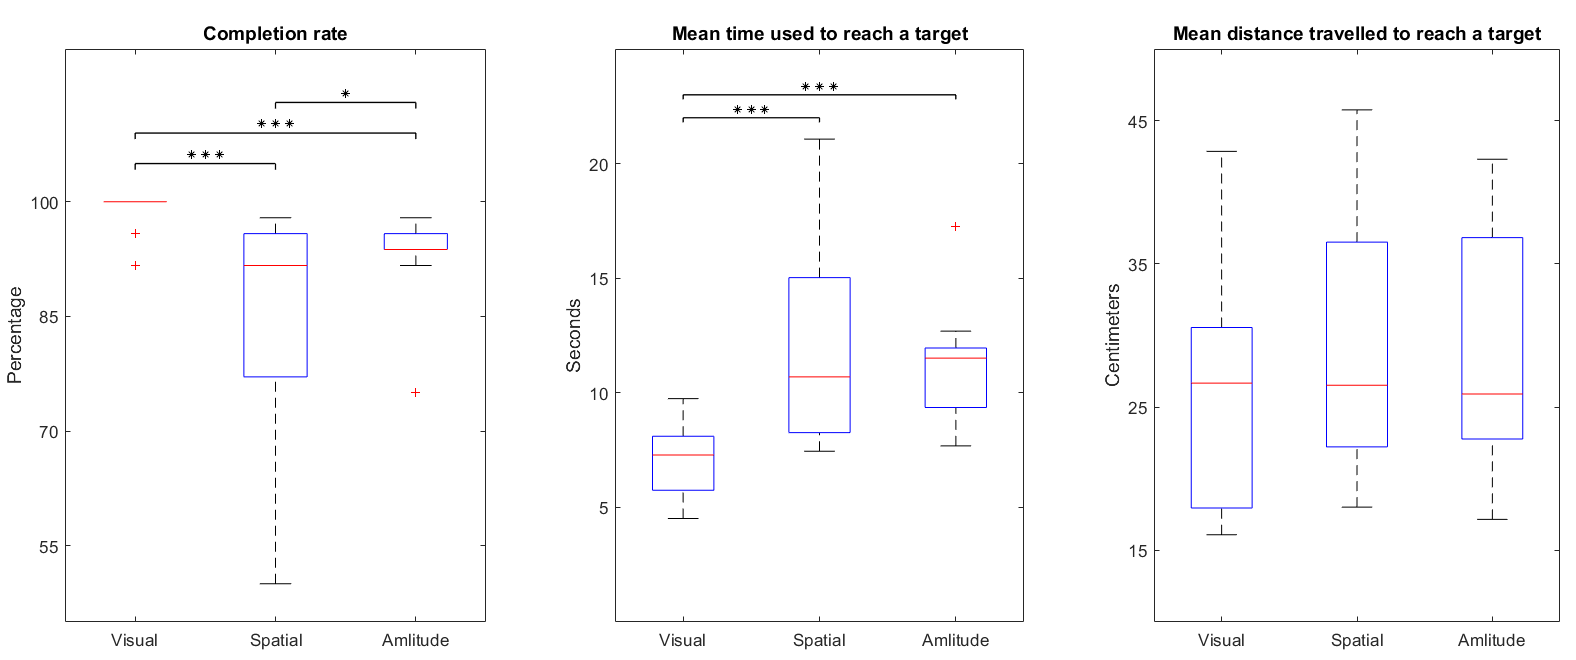
\includegraphics[width=0.9\textwidth]{figures/boxplot_results}
	\caption{Box plots of the metrics extracted from the visual, spatial and amplitude feedback evaluation tests. The two evaluation tests in the spatial and amplitude feedback block, respectively, were combined by calculating the mean between the two tests. One asterisk indicates p-value < 0.05 and three asterisks indicates p-value < 0.001.}
	\label{fig:pa:boxplot_results} 
\end{figure*}

\begin{figure}[H]                 
	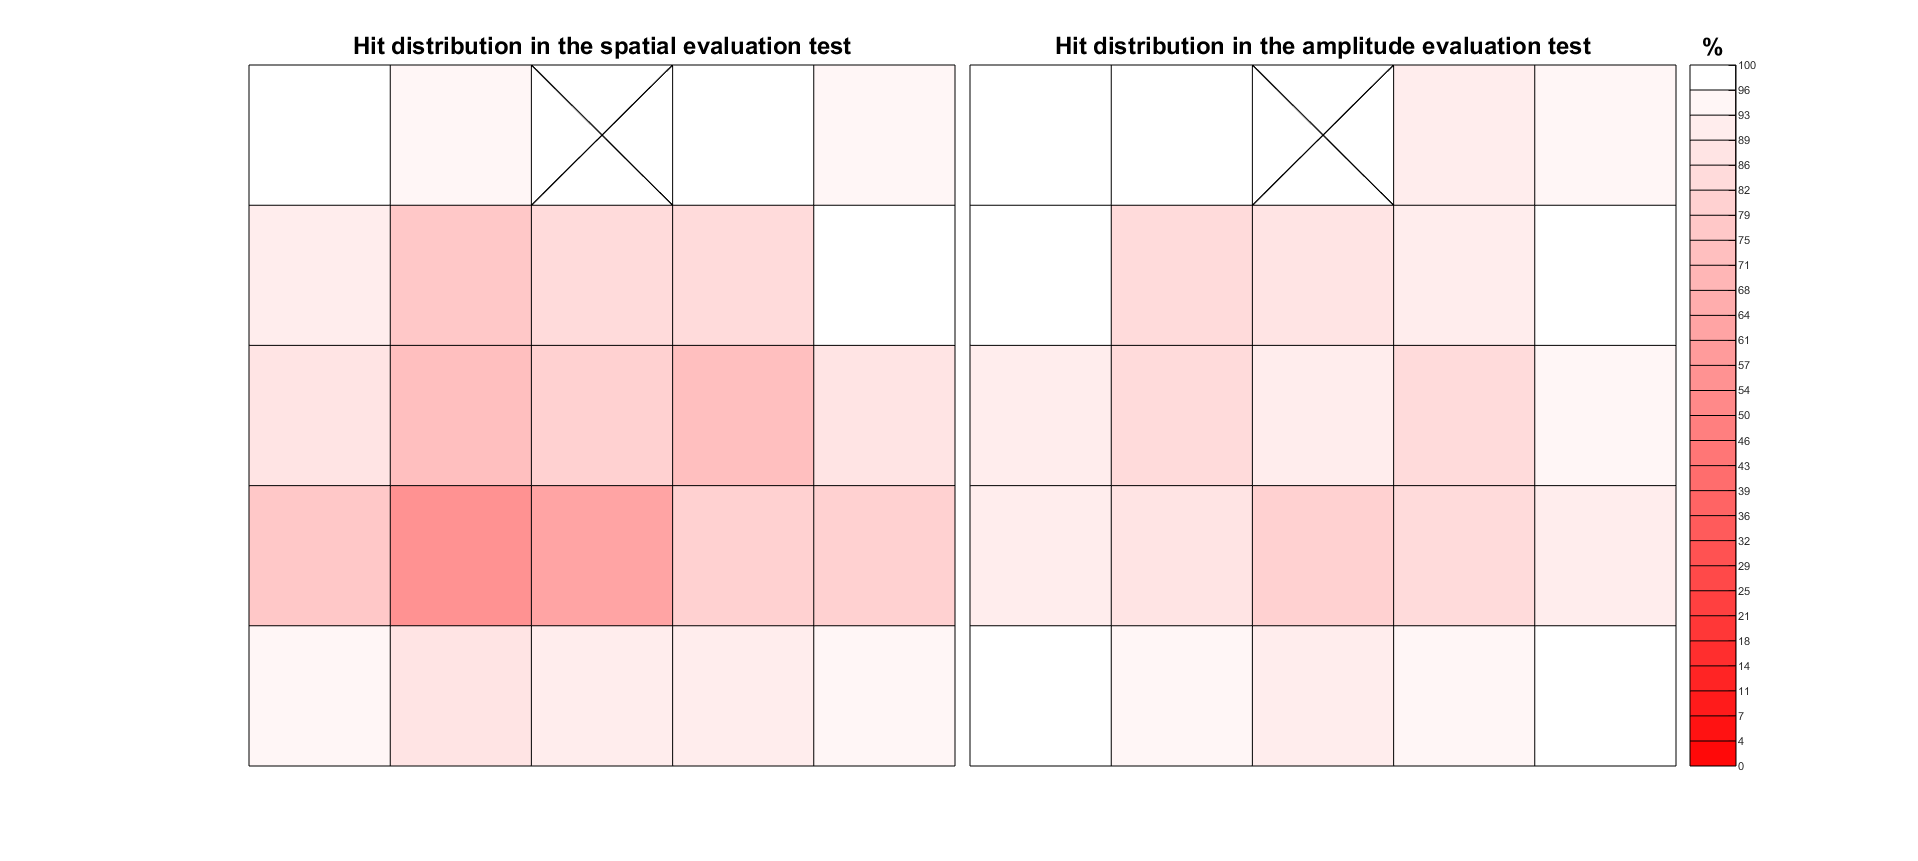
\includegraphics[width=.7\textwidth]{figures/hit_dist}
	\caption{Hit rate for each target in the spatial and amplitude evaluation test, respectively. The more transparent a target is, the higher the hit rate was. 100 $\%$ accounts for a total of 28 hits for each test.}
	\label{fig:pa:hit_dist} 
\end{figure}


